\section{测度的差}
\label{sec:measure-signed}

上一节只问两种测度是否忽略相同的集合。若要知道它们在每个集合上差多少，最直接的办法是作差：对两个有限测度$\nu,\mu$，令$\eta(A)=\nu(A)-\mu(A)$。这个赋值可以为正，也可以为负。本节研究这类赋值：它在哪里取正、在哪里取负，能否唯一地写回两个非负测度之差，以及怎样度量它的变化总量。积分尚未定义，本节不讨论对有符号测度的积分。

\subsection{有限有符号测度}
\label{sec:measure-signed-finite}

\paragraph{从测度之差到有符号赋值}
设$\nu,\mu$是$(X,\mathcal A)$上的有限测度，$\eta=\nu-\mu$。对两两不交的可测集$A_1,A_2,\dots$，两个测度各自可数可加，且两个级数都收敛到有限值，所以
\[
 \eta\Bigl(\bigcup_nA_n\Bigr)=\sum_n\nu(A_n)-\sum_n\mu(A_n)=\sum_n\bigl(\nu(A_n)-\mu(A_n)\bigr)=\sum_n\eta(A_n).
\]
可见$\eta$保留了可数可加性，只是不再非负。把这两条性质单独抽出来，就得到下面的定义。

\begin{definition}[有限有符号测度]
\label{def:measure-signed}
可测空间$(X,\mathcal A)$上的\term{有符号测度}（signed measure）$\eta$是映射$\eta:\mathcal A\to\mathbb R$，满足$\eta(\varnothing)=0$，并且对任意两两不交的$A_1,A_2,\dots\in\mathcal A$，级数$\sum_n\eta(A_n)$收敛且
\[
 \eta\Bigl(\bigcup_{n=1}^\infty A_n\Bigr)=\sum_{n=1}^\infty\eta(A_n).
\]
本书只讨论取有限实值的情形，称为有限有符号测度。
\end{definition}

不交集合的并与排列次序无关，所以上式右端的级数无论怎样重排都收敛到同一个值；按实数级数的重排定理，这意味着它绝对收敛。本章后面只用到一个更弱的推论：级数收敛，其通项必须趋于零。

有符号测度是给\emph{集合}赋予实数的规则，不要与在某些\emph{点}上取负值的实值函数混淆。$\eta(A)<0$表示集合$A$上的“负质量”多于“正质量”，这个数由整个集合决定，而不是由某一点的取值决定。要求取有限值，是为了避免出现$+\infty-\infty$：两个无限测度作差时，$\nu(A)-\mu(A)$可能根本没有定义。

\begin{example}[正负抵消]
\label{ex:measure-signed-weights}
取$X=\{1,2,3,4\}$及全部子集，规定单点值
\[
 \eta(\{1\})=2,\quad \eta(\{2\})=-1,\quad \eta(\{3\})=1,\quad \eta(\{4\})=-2,
\]
并令$\eta(A)=\sum_{i\in A}\eta(\{i\})$。有限集上的这种加和自动满足可加性，所以$\eta$是有符号测度；它也可以写成$\eta=\nu-\mu$，其中$\nu=2\delta_1+\delta_3$，$\mu=\delta_2+2\delta_4$。

计算几个值：$\eta(X)=2-1+1-2=0$，$\eta(\{1,2\})=1$，$\eta(\{1,3\})=3$，$\eta(\{2,4\})=-3$。全空间上的值为零，但这只是正负抵消的结果；在$\{1,3\}$与$\{2,4\}$上，$\eta$的绝对值都达到$3$。所以$\eta(X)$很小甚至为零，不能说明$\eta$在各处都小。图~\ref{fig:measure-signed-weights}把四个权重画成向上、向下的柱。
\end{example}

\begin{figure}[!htbp]
  \centering
  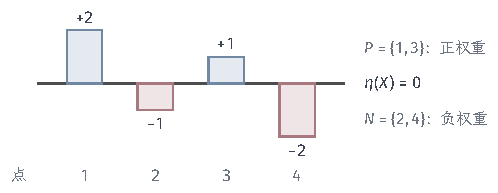
\includegraphics[width=84.36mm]{figures/02-abstract-mathematics/01-metric-and-measure/tikz/c2-signed-weights/figure.pdf}
  \caption{四点集合上的有符号测度。蓝色柱向上表示正权重，红色柱向下表示负权重。正负相互抵消使$\eta(X)=0$，但$\eta$在$P=\{1,3\}$上为$3$，在$N=\{2,4\}$上为$-3$。}
  \label{fig:measure-signed-weights}
\end{figure}

例中的$\eta$还有另一种写法：$\eta=(\nu+\delta_1)-(\mu+\delta_1)$。同一个有符号测度可以有许多种“正测度减正测度”的表示。下一小节要找的是其中一种由$\eta$本身确定、没有多余抵消的表示。

\subsection{Hahn分解与Jordan分解}
\label{sec:measure-hahn-jordan}

例~\ref{ex:measure-signed-weights}中，只要把$X$分成$\{1,3\}$与$\{2,4\}$，$\eta$在前一部分的每个子集上都非负，在后一部分的每个子集上都非正。一般的有符号测度是否也能这样一刀切成正、负两个区域？这正是Hahn分解回答的问题。

\paragraph{正集与负集}
只看$\eta(P)\ge0$并不够：在例~\ref{ex:measure-signed-weights}中$\eta(\{1,2\})=1\ge0$，但它的子集$\{2\}$取值为$-1$。我们需要的是对所有子集都保持符号的集合。

\begin{definition}[正集与负集]
\label{def:measure-positive-set}
设$\eta$是$(X,\mathcal A)$上的有限有符号测度。若$P\in\mathcal A$的每个可测子集$E$都满足$\eta(E)\ge0$，称$P$为$\eta$的\term{正集}（positive set）；若$N\in\mathcal A$的每个可测子集$E$都满足$\eta(E)\le0$，称$N$为$\eta$的\term{负集}（negative set）。
\end{definition}

正集的可测子集仍是正集，可数个正集的并也是正集：若$P_1,P_2,\dots$是正集，$E\subseteq\bigcup_nP_n$可测，令$E_1=E\cap P_1$，$E_n=E\cap P_n\setminus(P_1\cup\dots\cup P_{n-1})$，则$E_n$是$P_n$的可测子集且两两不交，$\eta(E)=\sum_n\eta(E_n)\ge0$。负集同理。

\paragraph{两条准备性质}
构造正负区域之前，需要两条只依赖可数可加性的性质。第一条说明有限有符号测度的取值不会无限地向下（或向上）延伸，这样“使$\eta$最小的集合”才有可能存在；第二条把测度的单调集合列连续性搬到有符号情形。

\begin{lemma}[有限有符号测度有界]
\label{lem:measure-signed-bounded}
有限有符号测度$\eta$有界：存在$M<\infty$，使$|\eta(A)|\le M$对一切$A\in\mathcal A$成立。
\end{lemma}

\begin{proof}
称可测集$A$是\emph{无界的}，如果$\sup\{|\eta(E)|:E\subseteq A,\ E\in\mathcal A\}=\infty$。设结论不成立，即$X$是无界的。我们将构造两两不交的可测集$B_1,B_2,\dots$，使每个$|\eta(B_n)|\ge1$。

设$A$是无界集。取可测子集$E\subseteq A$使$|\eta(E)|\ge|\eta(A)|+1$，则
\[
 |\eta(A\setminus E)|=|\eta(A)-\eta(E)|\ge|\eta(E)|-|\eta(A)|\ge1 .
\]
于是$E$与$A\setminus E$的取值绝对值都至少为$1$。它们中至少有一个是无界的：否则$A$的任一可测子集$F$满足$|\eta(F)|\le|\eta(F\cap E)|+|\eta(F\setminus E)|$，右边两项都有界，$A$就不是无界的。把无界的那一块记为$A'$，另一块记为$B$，则$B\subseteq A\setminus A'$且$|\eta(B)|\ge1$。

从$A_0=X$出发反复执行这一步，得到无界集$A_0\supseteq A_1\supseteq\cdots$及$B_n\subseteq A_{n-1}\setminus A_n$。由于$B_n\subseteq A_{n-1}\setminus A_n$，而$B_m\subseteq A_{m-1}\subseteq A_n$（$m>n$），这些$B_n$两两不交。按定义~\ref{def:measure-signed}，$\sum_n\eta(B_n)$收敛到$\eta(\bigcup_nB_n)$，通项必须趋于零；但$|\eta(B_n)|\ge1$，矛盾。
\end{proof}

\begin{lemma}[有符号测度的单调连续性]
\label{lem:measure-signed-continuity}
设$\eta$是有限有符号测度。若$A_1\subseteq A_2\subseteq\cdots$，则$\eta(\bigcup_nA_n)=\lim_n\eta(A_n)$；若$A_1\supseteq A_2\supseteq\cdots$，则$\eta(\bigcap_nA_n)=\lim_n\eta(A_n)$。
\end{lemma}

\begin{proof}
对递增集合列，令$D_1=A_1$，$D_n=A_n\setminus A_{n-1}$，它们两两不交，$\bigcup_nA_n=\bigcup_nD_n$，且$A_n=D_1\cup\dots\cup D_n$。由可数可加性，$\eta(\bigcup_nA_n)=\sum_n\eta(D_n)$，部分和恰为$\eta(A_n)$，所以等式成立。对递减集合列，$A_1\setminus A_n$递增，并为$A_1\setminus\bigcap_nA_n$；由已证部分及有限可加性$\eta(A_1\setminus B)=\eta(A_1)-\eta(B)$（$B\subseteq A_1$，各项有限），得$\eta(A_1)-\eta(\bigcap_nA_n)=\lim_n(\eta(A_1)-\eta(A_n))$。
\end{proof}

与非负测度不同，这里递减情形不需要另加有限性假设，因为$\eta$本身只取有限值。

\paragraph{Hahn分解}
思路是寻找使$\eta$取最小值的可测集$D$。若某个$D$达到最小值，那么从$D$中拿走一个正值子集，或向$D$中添入一个负值的外部集合，都会让取值更小，这不可能；于是$D$自然是负集，补集是正集。难点在于证明最小值确实能被某个集合达到。

\begin{theorem}[Hahn分解]
\label{thm:measure-hahn}
设$\eta$是$(X,\mathcal A)$上的有限有符号测度。则存在$P\in\mathcal A$，使$P$是$\eta$的正集，$N=X\setminus P$是$\eta$的负集。这样的一对$(P,N)$称为$\eta$的\term{Hahn分解}（Hahn decomposition）。若$(P',N')$是另一组Hahn分解，则$P\cap N'$与$P'\cap N$的每个可测子集上$\eta$都取零。
\end{theorem}

\begin{proof}
令$m=\inf_{A\in\mathcal A}\eta(A)$。由引理~\ref{lem:measure-signed-bounded}，$m$是有限实数；又$\eta(\varnothing)=0$，故$m\le0$。对每个$n$取可测集$A_n$使$\eta(A_n)<m+2^{-n}$。

第一步说明两个“近乎最小”的集合取交后仍近乎最小。对可测集$A,B$，有限可加性给出$\eta(A\cup B)+\eta(A\cap B)=\eta(A)+\eta(B)$；又$\eta(A\cup B)\ge m$，所以
\[
 \eta(A\cap B)\le\eta(A)+\eta(B)-m .
\]
固定$n$，对$k\ge n$令$C_{n,k}=A_n\cap A_{n+1}\cap\dots\cap A_k$。对$k$归纳，并利用上式，
\[
 \eta(C_{n,k+1})\le\eta(C_{n,k})+\eta(A_{k+1})-m<m+\sum_{j=n}^{k+1}2^{-j}.
\]
所以$\eta(C_{n,k})<m+2^{1-n}$对所有$k\ge n$成立。

第二步取极限。$C_{n,k}$关于$k$递减，令$C_n=\bigcap_{k\ge n}A_k$；由引理~\ref{lem:measure-signed-continuity}，$\eta(C_n)=\lim_k\eta(C_{n,k})\le m+2^{1-n}$。$C_n$关于$n$递增，令$D=\bigcup_nC_n$；再由引理~\ref{lem:measure-signed-continuity}，$\eta(D)=\lim_n\eta(C_n)\le m$。另一方面$\eta(D)\ge m$，所以$\eta(D)=m$，最小值被$D$达到。

第三步验证符号。若可测集$E\subseteq D$满足$\eta(E)>0$，则$\eta(D\setminus E)=m-\eta(E)<m$，与$m$是下确界矛盾，所以$D$是负集。若可测集$E\subseteq X\setminus D$满足$\eta(E)<0$，则$\eta(D\cup E)=m+\eta(E)<m$，同样矛盾，所以$X\setminus D$是正集。取$N=D$，$P=X\setminus D$即可。

最后看两组分解的差别。$P\cap N'$既是正集$P$的子集，又是负集$N'$的子集，它的每个可测子集$E$同时满足$\eta(E)\ge0$与$\eta(E)\le0$，即$\eta(E)=0$。$P'\cap N$同理。
\end{proof}

整个证明只用了集合运算、有限可加性与单调连续性。Hahn分解一般不唯一：$\eta$在其上“完全为零”的区域可以划给任意一侧。例如在实轴上令$\eta=\lambda|_{[0,1]}-\lambda|_{[2,3]}$，$P_1=(-\infty,3/2)$与$P_2=(-\infty,2)$都给出Hahn分解，两者相差的$[3/2,2)$上$\eta$的每个子集都取零，见图~\ref{fig:measure-hahn-decomposition}。正区域还可以只差一个Lebesgue零测集，例如把点$1/2$从$P_1$移到负区域一侧。

\begin{figure}[!htbp]
  \centering
  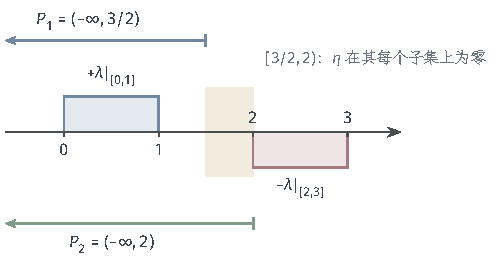
\includegraphics[width=84.06mm]{figures/02-abstract-mathematics/01-metric-and-measure/tikz/c2-hahn-decomposition/figure.pdf}
  \caption{Hahn分解的区域选择不唯一。$\eta=\lambda|_{[0,1]}-\lambda|_{[2,3]}$，蓝块在$[0,1]$上表示正的长度，红块在$[2,3]$上表示负的长度，块高表示长度测度前的系数$\pm1$。正区域可以取$P_1=(-\infty,3/2)$，也可以取$P_2=(-\infty,2)$；二者之差$[3/2,2)$（黄色）的每个可测子集上$\eta$都为零，所以放在哪一侧都不改变符号要求。}
  \label{fig:measure-hahn-decomposition}
\end{figure}

\paragraph{Jordan分解}
区域可以不同，但限制在区域上的质量却是唯一的。把$\eta$分别限制到正区域与负区域，就得到两个非负测度。

\begin{theorem}[Jordan分解]
\label{thm:measure-jordan}
设$\eta$是有限有符号测度，$(P,N)$是它的一组Hahn分解。令
\[
 \eta^+(A)=\eta(A\cap P),\qquad \eta^-(A)=-\eta(A\cap N),\qquad A\in\mathcal A .
\]
则$\eta^+,\eta^-$是有限非负测度，$\eta=\eta^+-\eta^-$，且$\eta^+\perp\eta^-$；它们不依赖于Hahn分解的选取。反过来，若$\eta=\alpha-\beta$，其中$\alpha,\beta$是相互奇异的有限非负测度，则$\alpha=\eta^+$，$\beta=\eta^-$。这个唯一的表示称为$\eta$的\term{Jordan分解}（Jordan decomposition），$\eta^+$、$\eta^-$分别称为$\eta$的正部分与负部分。
\end{theorem}

\begin{proof}
$A\cap P$是正集的子集，所以$\eta^+(A)\ge0$；同理$\eta^-(A)\ge0$。两者的可数可加性直接来自$\eta$：若$A_n$两两不交，则$A_n\cap P$也两两不交。由$A=(A\cap P)\cup(A\cap N)$得$\eta(A)=\eta^+(A)-\eta^-(A)$。又$\eta^+(N)=\eta(\varnothing)=0$，$\eta^-(X\setminus N)=\eta^-(P)=0$，所以$\eta^+\perp\eta^-$。

再看与Hahn分解无关。设$(P',N')$是另一组分解。由定理~\ref{thm:measure-hahn}，$A\cap P\cap N'$与$A\cap P'\cap N$上$\eta$取零，因此
\[
 \eta(A\cap P)=\eta(A\cap P\cap P')+\eta(A\cap P\cap N')=\eta(A\cap P\cap P')=\eta(A\cap P'),
\]
最后一步对$P'$作同样的拆分。$\eta^-$同理。

最后证唯一性。设$\eta=\alpha-\beta$且$\alpha\perp\beta$，按定义~\ref{def:measure-singular}取可测集$S$使$\beta(S)=0$，$\alpha(X\setminus S)=0$。对$S$的可测子集$E$，$\eta(E)=\alpha(E)-\beta(E)=\alpha(E)\ge0$；对$X\setminus S$的可测子集$E$，$\eta(E)=-\beta(E)\le0$。所以$(S,X\setminus S)$本身是一组Hahn分解。由已证的无关性，
\[
 \eta^+(A)=\eta(A\cap S)=\alpha(A\cap S)=\alpha(A),
\]
其中最后一步用了$\alpha(A\setminus S)=0$。同理$\beta=\eta^-$。
\end{proof}

Jordan分解的唯一性依赖“相互奇异”这一条件。任意两个有限测度之差都是有符号测度，但一般不是Jordan分解。仍取$\eta=\lambda|_{[0,1]}-\lambda|_{[2,3]}$，它的Jordan部分是$\eta^+=\lambda|_{[0,1]}$、$\eta^-=\lambda|_{[2,3]}$。另一方面，令
\[
 \alpha=\lambda|_{[0,3]},\qquad \beta=\lambda|_{[1,2]}+2\lambda|_{[2,3]},
\]
逐段检查：在$[0,1]$上$\alpha-\beta$的系数为$1-0=1$，在$[1,2]$上为$1-1=0$，在$[2,3]$上为$1-2=-1$，所以同样有$\alpha-\beta=\eta$。但$\alpha$与$\beta$在$[1,3]$上重叠，并不相互奇异，且$\alpha(\mathbb R)=\beta(\mathbb R)=3$，而$\eta^\pm(\mathbb R)=1$，见图~\ref{fig:measure-jordan-decomposition}。

这种多余的重叠总是只增不减。对任意表示$\eta=\alpha-\beta$（$\alpha,\beta$为有限非负测度）及任意$A\in\mathcal A$，
\[
 \eta^+(A)=\eta(A\cap P)=\alpha(A\cap P)-\beta(A\cap P)\le\alpha(A\cap P)\le\alpha(A),
\]
同理$\eta^-(A)\le\beta(A)$。所以Jordan分解是所有“正测度减正测度”表示中最小的一个。取$\alpha=\eta^+$时等号成立，于是还得到正部分的一个不依赖于Hahn分解的读法：
\[
 \eta^+(A)=\sup\{\eta(E):E\subseteq A,\ E\in\mathcal A\},
\]
因为每个$\eta(E)=\eta^+(E)-\eta^-(E)\le\eta^+(E)\le\eta^+(A)$，而$E=A\cap P$达到这个上界。

\begin{figure}[!htbp]
  \centering
  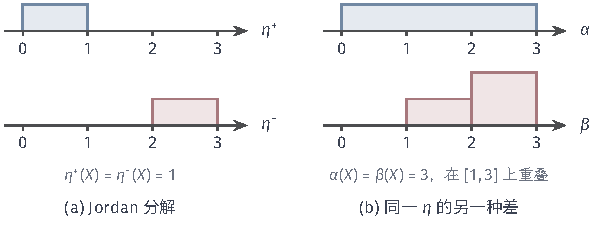
\includegraphics[width=101.745mm]{figures/02-abstract-mathematics/01-metric-and-measure/tikz/c2-jordan-decomposition/figure.pdf}
  \caption{同一个有符号测度$\eta=\lambda|_{[0,1]}-\lambda|_{[2,3]}$的两种差表示，块高为长度测度前的系数。(a)Jordan分解：$\eta^+$与$\eta^-$分别集中在$[0,1]$与$[2,3]$上，相互奇异，总质量各为$1$。(b)$\alpha=\lambda|_{[0,3]}$与$\beta=\lambda|_{[1,2]}+2\lambda|_{[2,3]}$之差也等于$\eta$，但两者在$[1,3]$上重叠，总质量各为$3$。}
  \label{fig:measure-jordan-decomposition}
\end{figure}

\subsection{总变差测度}
\label{sec:measure-total-variation}

$|\eta(A)|$衡量的是集合$A$上正负相抵后的净值；例~\ref{ex:measure-signed-weights}说明它可能掩盖很大的局部变化。若要累计正负两方面的全部质量，就应当把正部分与负部分相加，而不是相减。

\paragraph{定义与分割刻画}

\begin{definition}[总变差测度]
\label{def:measure-total-variation}
设$\eta$是有限有符号测度，$\eta=\eta^+-\eta^-$是它的Jordan分解。称
\[
 |\eta|=\eta^++\eta^-
\]
为$\eta$的\term{总变差测度}（total variation measure），称$|\eta|(X)$为$\eta$的总变差。
\end{definition}

$|\eta|$是两个有限非负测度之和，所以仍是有限非负测度。它也可以不借助Jordan分解，而直接从$\eta$的取值读出：把$A$切成有限块，对每块的净值取绝对值再相加，切得越合适，抵消越少。

\begin{theorem}[总变差的分割刻画]
\label{thm:measure-total-variation-partition}
对每个$A\in\mathcal A$，
\[
 \begin{aligned}
  |\eta|(A)=\sup\Bigl\{\sum_{i=1}^k|\eta(A_i)|:\ &k\ge1,\ A_1,\dots,A_k\in\mathcal A\text{两两不交},\\
  &\bigcup_{i=1}^kA_i=A\Bigr\}.
 \end{aligned}
\]
\end{theorem}

\begin{proof}
对$A$的任一有限可测分割，
\[
 \sum_i|\eta(A_i)|=\sum_i|\eta^+(A_i)-\eta^-(A_i)|\le\sum_i\bigl(\eta^+(A_i)+\eta^-(A_i)\bigr)=|\eta|(A),
\]
最后一步用了$\eta^\pm$的有限可加性。所以上确界不超过$|\eta|(A)$。取Hahn分解$(P,N)$及分割$A_1=A\cap P$、$A_2=A\cap N$，则$|\eta(A_1)|+|\eta(A_2)|=\eta^+(A)+\eta^-(A)=|\eta|(A)$，上确界被达到。
\end{proof}

回到例~\ref{ex:measure-signed-weights}。不分割时$|\eta(X)|=0$；分成$\{1,2\}$与$\{3,4\}$时得$|1|+|-1|=2$；分成$\{1,3\}$与$\{2,4\}$时得$|3|+|-3|=6$。再细分也不会超过$6$，因为四个单点上的绝对值之和为$2+1+1+2=6$。所以$|\eta|(X)=6$，正好由正负区域的分割取得，见图~\ref{fig:measure-total-variation-partition}。

\begin{figure}[!htbp]
  \centering
  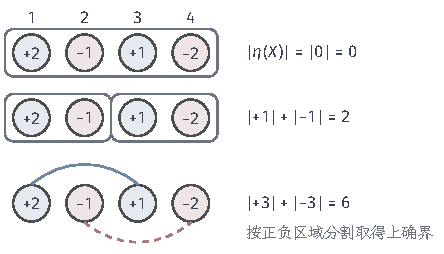
\includegraphics[width=75.128mm]{figures/02-abstract-mathematics/01-metric-and-measure/tikz/c2-total-variation-partition/figure.pdf}
  \caption{用分割读取总变差。四个点的权重为$+2,-1,+1,-2$。第一行不分割，净值为$0$；第二行把相邻的正负点合在一起，仍有抵消，绝对值之和为$2$；第三行按符号分组（蓝色实弧连接正点，红色虚弧连接负点），没有抵消，绝对值之和为$6=|\eta|(X)$。}
  \label{fig:measure-total-variation-partition}
\end{figure}

\paragraph{净值与总量}
由分割刻画取平凡分割$\{A\}$，立即得到
\[
 |\eta(A)|\le|\eta|(A),\qquad A\in\mathcal A .
\]
左边允许抵消，右边累计正负变化的总量。特别地，$|\eta|(A)=0$当且仅当$\eta$在$A$的每个可测子集上都取零：必要性来自上面的不等式用于子集，充分性来自分割刻画中每一项都为零。因此$|\eta|$的零测集正是$\eta$“完全看不见”的集合；后面讨论有符号测度时，“几乎处处”都相对于$|\eta|$来理解。

对两个概率测度$P,Q$，差$\eta=P-Q$满足$\eta(X)=0$，于是$\eta^+(X)=\eta^-(X)=\tfrac12|\eta|(X)$；再由正部分的上确界读法，
\[
 \tfrac12|P-Q|(X)=\eta^+(X)=\sup_{A\in\mathcal A}\bigl(P(A)-Q(A)\bigr).
\]
这个量在后续比较概率分布时称为全变差距离，它与其他分布距离的关系留到讨论概率分布的部分。第~\ref{chap:integration}章将用$|\eta|$为有符号测度的积分规定绝对可积条件，第~\ref{chap:densities-change-of-measure}章则研究$\eta$何时能由一个可积函数表示。
